%%%%%%%%%%%%%%%%%%%%%%%%%%%%%%%%%%%%%%%%%%%%%%%%%%%%%%%%%%%%%%%%%%%%%%%%%%%%%%%%
%2345678901234567890123456789012345678901234567890123456789012345678901234567890
%  1  2  3  4  5  6  7  8

\documentclass[letterpaper, 11 pt, conference]{ieeeconf} % Comment this line out
          % if you need a4paper
%\documentclass[a4paper, 10pt, conference]{ieeeconf} % Use this line for a4
          % paper

\IEEEoverridecommandlockouts     % This command is only
          % needed if you want to
          % use the \thanks command
\overrideIEEEmargins
% See the \addtolength command later in the file to balance the column lengths
% on the last page of the document
\renewcommand{\baselinestretch}{1.0}

\pagenumbering{arabic}

% The following packages can be found on http:\\www.ctan.org
\usepackage{graphicx} % for pdf, bitmapped graphics files
%\usepackage{epsfig} % for postscript graphics files
%\usepackage{mathptmx} % assumes new font selection scheme installed
%\usepackage{times} % assumes new font selection scheme installed
%\usepackage{amsmath} % assumes amsmath package installed
%\usepackage{amssymb} % assumes amsmath package installed
\usepackage{enumitem}
\usepackage{float}
\usepackage{lipsum}
\usepackage{caption}
\usepackage{cite}
\usepackage{spreadtab}

\captionsetup[table]{position=bottom}

\title{\LARGE \bf
Flexible needle and patient tracking using fractional scanning for reduced dose in interventional CT procedures
}

\author{Guy Medan and Leo Joskowicz, Fellow, IEEE% <-this % stops a space
\thanks{Research supported by Kamin grant 57706, Office of the Chief Scientist, Ministry of Trade and Industry, Israel. We thank Eyal Lin and Ronen Shter of GE Healthcare Israel for the CT scans and for their valuable assistance.}% <-this % stops a space
\thanks{G. Medan and L. Joskowicz are with the CASMIP Laboratory, School of Computer Science and Engineering, The Hebrew University of Jerusalem, Israel (josko@cs.huji.ac.il).}%
}

\renewcommand{\citepunct}{,\penalty\citepunctpenalty\,}
\renewcommand{\citedash}{--} 
\begin{document}


\maketitle
\thispagestyle{plain}
\pagestyle{plain}


%%%%%%%%%%%%%%%%%%%%%%%%%%%%%%%%%%%%%%%%%%%%%%%%%%%%%%%%%%%%%%%%%%%%%%%%%%%%%%%%
\begin{abstract}
We present a new method for image-less flexible needle and patient tracking in interventional CT procedures based on fractional CT scanning, extending a previous method for rigid needles.
Our method accurately localizes the trajectory of a flexible needle to which a spherical marker is attached at a known distance from the tip with respect to a baseline scan of patient in the CT scanner coordinate frame. 
This is achieved with lower dose compared to a full scan using sparse view angle sampling and without reconstructing the CT image.
Our method takes advantage of rigid registration to the baseline scan computed from the sparse projection data to calculate projection difference images, in which the needle and attached spherical marker are prominent features, allowing the needle trajectory to be traced in 3D space from its 2D projections.
We performed registration and needle trajectory localization in seven abdomen phantom scans using two kinds of flexible needles, and obtained an average of 2.4 mm tip localization error.
The dose reduction enables more frequent needle trajectory localizations during needle insertion for a similar total dose, or a reduced total dose for the same frequency of localization.

\end{abstract}

\begin{keywords}
interventional CT, fractional CT scanning, reduced dose CT scanning, flexible needle tracking, radon space registration 
\end{keywords}

%%%%%%%%%%%%%%%%%%%%%%%%%%%%%%%%%%%%%%%%%%%%%%%%%%%%%%%%%%%%%%%%%%%%%%%%%%%%%%%%
\section{Introduction}

Image guided minimally invasive techniques have become commonplace for interventional procedures such as biopsies and aspirations.
In these procedures a flexible needle is inserted under image guidance toward a target, either manually or using robotic actuators. Repeated imaging is acquired during insertion in order to verify the needle is advancing in the desired direction, as errors in needle placement can lead to wrong diagnosis or failed treatment.

CT guidance is often used in interventional radiology procedures.
While providing high resolution volumetric imaging of the patient, CT-guided interventions also carry several limitations and drawbacks.
The intervention protocol typically requires the needle to be aligned with the axial plane of imaging as it is being inserted \cite{gupta2014ct}, which requires careful positioning of the patient to allow access to the target.
Additionally, the presence of the needle in the scanned volume introduces image artifacts, due to beam hardening and scatter \cite{boas2012ctartifacts}, which can obscure important anatomical structures near the needle tip.
And finally, the patient's exposure to accumulating ionizing X-ray radiation may increase the risk of cancer \cite{mettler2000ct, chodick2007excess}, which is exacerbated in interventional CT due to the number of repeat scans acquired during the procedure.

Other imaging modalities used for interventional procedures include ultrasound, fluoroscopy and cone-beam CT.
Ultrasound is a cost effective imaging solution, though it provides only 2D cross sections at limited resolution and signal-to-noise ratio (SNR) \cite{sheafor2000comparison}.
Fluoroscopy offers improved spatial resolution, but is not suitable when complex anatomical relationships must be characterized in 3D during the intervention.
Flat-panel cone-beam CT is a relatively new technology increasingly used in interventional radiology, although it suffers from longer scan times and increased radiation scatter, resulting in increased artifacts compared to multi-detector CT \cite{orth2008cbct}.

Dose reduction techniques for CT mainly focus on achieving a good quality of reconstruction within the context of a single acquisition by scanning with lower tube current, resulting in lowered SNR, which is overcome by denoising \cite{manduca2009projection} or using statistical noise models in the reconstruction of the image \cite{zhang2016statistical,kim2015sparseview,niu2014sparse,liu2014total}. 

However, in the common cases where a full baseline scan (without the needle) is available, a different approach can be used:
selective acquisition of a sparse set of projection views, referred to as fractional scanning, enables reducing the radiation dose by modulating the source of x-rays during its rotation. By exploiting the projection space raw data, registration with the baseline scan and localization of the needle in the repeat scan can be achieved without reconstruction of the repeat scan image \cite{medan2017sparse, medan2017reduced}.

\section{Previous work}
Different methods have been proposed to achieve accurate needle insertion by robotic actuators, with work focused on mechanical modelling of the system, environment and trajectory planning, but with little attention to needle localization from imaging modalities as feedback.
Works by Wu et al. \cite{wu2013automatic} and Engh et al. \cite{engh2010percutaneous} describe implementations of a bevel-tip needle steering method using duty-cycle spinning of the needle, relying on its bending tendency due to asymmetry. Such systems model the needle-tissue interaction to execute a control sequence achieving a pre-planned trajectory. Imaging-based feedback is mentioned as a means to allow corrections of the control sequence mid-insertion by adjusting the planned trajectory based on the actual needle trajectory.
Ben-David et al. \cite{ben2018robotic} describe a robotic system for flexible needle insertion under CT guidance. A dual guiding mechanism is composed of a driver which advances the needle while a positioning unit steers it during insertion. A pre-planned 3D trajectory is executed and amended during the insertion based on full repeated CT scans.
Earlier work by Glozman et al. \cite{glozman2007image} describes robotic flexible needle steering and a needle-tissue mechanical interaction model, where feedback is based on 2D in-plane imaging of the needle.

Most works in needle localization from medical images use ultrasound as the imaging modality. A robotically positioned 2D transducer perpendicular to the needle tip is by presented Vrooijink et al. \cite{vrooijink2013real}, where needle-induced image artifacts are taken advantage of in order to localize the needle tip in the imaged plane, while the transducer is continuously re-positioned to maintain its orientation relative to the needle tip. An approach combining both ultrasound and CT fluoroscopy is presented in \cite{marinetto2017integration}, where a free-hand ultrasound probe and C-arm are registered using an external optical tracker to produce a fused image in which the needle can be tracked.

The following works describe specific methods to localize the needle path in reconstructed CT images:
Hou et al. \cite{huo2015shape} reconstruct the bevel-tip flexible needle path from full CT slices by localizing points at which the needle intersects slice planes, and fitting a four-order polynomial to the collection of 3D points.
Yaniv et al. \cite{yaniv2010needle} describe a system in which embedded electromagnetic fiducials are used for needle tracking under CT guidance, with operator input required to identify the needle tip in a full CT scan taken in-situ. These methods rely on acquisition of full repeat scan and reconstruction of the image for each localization of the needle. This approach carries the associated cost in radiation dose for the patient. In the following section, we present a novel imageless method for flexible needle localization in projection space using fractional scanning, which promises to reduce the radiation dose associated with each needle localization.

\section{Method}

We describe next an extension to flexible needles of our previous method \cite{medan2017reduced} for volume image-less rigid needle and patient tracking in interventional CT procedures based on fractional CT scanning. Similarly to our previous method, we begin by computing a sinogram-space rigid registration of the patient position in the CT scanner coordinate frame between a baseline scan without a needle, and a repeat scan with a needle introduced. The repeat scan is performed by sampling sparsely in the view angle domain (fractional scanning) and without reconstructing the CT image, while the baseline scan is assumed to be a full scan (sampled densely in the view angle domain). We use projection difference images (shown in fig. \ref{proj_diff_fig}), which are calculated by subtracting registered reprojected baseline scan images from the sparse set of repeat projection images. These highlight the differences between scans, which in our case is assumed to be the needle. The needle path is then traced in 3D space using only the projection difference images. The stages of our method are outlined below:
\begin{enumerate}
\item \textit{Fractional scanning}. A fractional repeat scan is obtained with the needle in place. The full baseline scan and fractional repeat scan are registered using our sinogram space rigid registration method \cite{medan2017sparse}.
\item \textit{Projection difference}. Using the obtained rigid registration, the projection difference images are calculated by applying the rigid transformation to the baseline scan volume, forward projection, and subtracting from corresponding repeat scan projection images. The images are then post-processed to enhance features that are locally similar to lines.
\item \textit{Spherical marker localization}. we obtain a 3D localization of a spherical marker attached to the needle at a known distance from the tip, using the projection difference images.
\item \textit{Incremental needle path tracing}. starting from the center of the marker obtained in the previous stage, we incrementally trace the needle path in 3D space using the projection difference images.
\item \textit{Display/feedback}. the current location of the needle with respect to the baseline scan 3D image is displayed and/or used as feedback for further driving the needle toward the target.
\end{enumerate}
Steps 1-5 are repeated each time the needle is further inserted during the intervention, until the tip localization shows the desired target structure inside the patient is reached. Optionally, full CT scans for image reconstruction can be acquired during the procedure as needed. Our method uses the same sparse projection sampling pattern both for registration and for needle localization, avoiding additional scanning and image reconstruction so the radiation dose is a fraction of that required in image based methods. This allows frequent needle insertion and localization for feedback and accuracy without excessive radiation dose.

The rest of this section is organized as follows.
Section \ref{markerloc} summarizes the step for localizing the spherical marker in 3D space.
Section \ref{inctracing} provides a detailed breakdown of the incremental 3D curve tracing algorithm.

\subsection{Marker localization} \label{markerloc}
The 3D center of the spherical marker is localized in three stages, using a method previously outlined in our method for rigid needles \cite{medan2017reduced}. 
First, the 2D centers of the projected spherical marker are roughly localized in each of the $K$ projection difference images by correlating the difference projection image with a circular pattern. 
Then, the 2D projected marker centers in each projection difference image are refined by optimizing a cost function which takes into account the image gradients of the marker's surface.
Finally, the 3D position of the marker center $s$ is calculated by solving an inverse problem using the known projection geometry of the CT and the localized marker centers.

\subsection{Incremental path tracing} \label{inctracing}

The path of the needle in 3D space is estimated by incrementally establishing a series of equidistant bezier curve control points along the path of the needle in 3D space $p_1, p_2, ..., p_i$, starting from the marker center $p_1=s$, which are used to construct a 3D curve $C_i$ tracing the path of the needle from the center of the spherical marker toward the tip, where $i$ is the number of control points in the incremental process. 

\begin{enumerate}
 \item Starting from the center of the spherical marker, the initial direction of the first needle segment is determined in 3D space using its 2D projections onto the projection difference images, by optimizing a cost function which is designed to attain a minimum when the projection difference images contain line segment in the projected direction. Four control points are placed at regular intervals along the initial segment.
 \item Starting from the end of the previous segment, the next segment direction is determined in 3D space in a similar manner, and one control point is placed at the new segment end.
 \item The process is repeated and the accumulated control points are used to evaluate a bezier curve in 3D space such that the sum squared distances of the control points from the curve is minimized.
 \item Once the length of the evaluated curve exceeds the known distance between the tip and the center of the spherical marker, the last segment is shortened accordingly, with the last point representing the tip localization.
\end{enumerate}

In each iteration a new point $p_{i+1}(\hat{n}) = p_i + \Gamma \hat{n}$ is sought, where $\Gamma$ is a fixed parameter for segment length, and $\hat{n}$ is a direction to be determined via optimization of a cost function detailed below.
A 3D curve $C_{i+1}[\hat{n}]$ is obtained from the control points $p_1, p_2, ..., p_i, p_{i+1}(\hat{n})$, and projected onto each of the $K$ view angles projection difference images to obtain projected curves $P_j C_{i+1}[\hat{n}] = c_{i+1}^j[\hat{n}]$ where $j=1,...,K$ is the view angle index and $P_j$ is the projection operator for view $j$.
The direction $\hat{n}$ is obtained by optimizing a cost function designed to attain a minimum when the projection of the curve $C_{i+1}$ onto the set of projection difference images follows the needle path traced in the images:
\[ \Psi_i(\theta, \phi) = -\sum_{j=1}^K{\int_{r \in c_{i+1}^j[\hat{n}(\theta, \phi)]} {I_j(r)dl}} \]
where $ \theta, \phi$ are spherical coordinates, $ \hat{n}(\theta, \phi) $ is the conversion from spherical coordinates to unit vector $ \hat{n} $, and $r$ is the 2D coordinate along the projected path $c_{i+1}^j[\hat{n}]$ in projection difference image $I_j$. 
Accordingly, the orientation of the $i$-th segment is obtained as $(\theta_i^*, \phi_i^*) = \textsf{argmin}_{\theta, \phi} \Psi_i ( \theta, \phi)$. Then, a new control point $p_{i+1}$ is added to the series of established control points $p_1, p_2, ..., p_i$ using the relation:
$$ p_{i+1} = p_i + \Gamma \hat{n}(\theta_i^*, \phi_i^*) $$

The incremental process is stopped once the length of the 3D curve $C_{i+1}$ exceeds the known distance between the marker and needle tip. Then, the tip position is determined by trimming the last segment so that the overall length of the curve is equal to the known marker-tip distance.

\begin{table}[t]
\begin{center}
\begin{tabular}{|c||c|c|c|c|}
\hline
Scan & Reg. error & Marker & Tip error & Trajectory\\
ID  & [mm] & error [mm] & [mm] & error  [mm]\\
\hline
\hline
L1 & 1.4 & 1.9 & 2.6 & 0.7\\
\hline
L2 & 0.7 & 0.8 & 1.9 & 0.6\\
\hline
L3 & 0.6 & 0.3 & 4.3 & 0.9 \\
\hline
L4 & 1.0 & 0.8 & 2.0 & 0.5\\
\hline
S1 & 1.4 & 1.1 & 2.4 & 0.5\\
\hline
S2 & 1.2 & 1.5 & 1.4 & 0.6\\
\hline
S3 & 1.5 & 0.9 & 2.2 & 0.9\\
\hline
\hline
L & 
0.9 \pm\hspace{0.1cm} 0.4 & 
1.0 \pm\hspace{0.1cm} 0.7 & 
2.7 \pm\hspace{0.1cm} 1.1 & 
0.7 \pm\hspace{0.1cm} 0.2\\
\hline
S & 
1.4 \pm\hspace{0.1cm} 0.2 &  
1.2 \pm\hspace{0.1cm} 0.3 & 
2.0 \pm\hspace{0.1cm} 0.5 &  
0.7 \pm\hspace{0.1cm} 0.2\\
\hline
ALL & 
1.1 \pm\hspace{0.1cm} 0.4 &  
1.0 \pm\hspace{0.1cm} 0.5 &  
2.4 \pm\hspace{0.1cm} 0.9 &  
0.7 \pm\hspace{0.1cm} 0.2\\
\hline
\end{tabular}
\caption{\small{Summary of experimental results. L/S stands for long/short needle, respectively.
The bottom part of the table shows means and standard deviations across the long, short and all scans in the dataset.}}
\label{results_table}
\end{center}
\end{table}


\section{Results}

To demonstrate our method we conducted an experiment consisting of flexible needles inserted into an abdomen phantom (CIRS model 57 Triple Modality 3D Abdominal Phantom) and scanned using GE Discovery CT750HD scanner at GE Healthcare Haifa (see fig. \ref{long_needle_fig}). The needles used were: a long 16 gauge (1.65mm outer diameter) needle, and short 22 gauge (0.72mm outer diameter) needle. For the long needle, the marker center was fixed at 235mm from the tip, and for the short needle at 135mm (figures \ref{long_needle_fig} and \ref{short_needle_fig} respectively).
The reconstructed image size is 800$\times$800$\times$144 voxels, with spatial resolution of 0.58$\times$0.58$\times$1.25 mm$^3$. The detector array consists of 885 elements scanned at 984 views at regular intervals in the range [0$^{\circ}$ , 360$^{\circ}$), where four slices were acquired in each full revolution. The data was re-binned from fan-beam to parallel rays representation of the projections.

At first a scan of the empty scanner bed was performed so that its sinogram can be subtracted from the following scans (this is done since the scanner bed does not undergo the same rigid movement as the phantom). Then, a full (i.e. dense sampling of view angles) baseline scan of the phantom was acquired, without the needle present. At each subsequent scan, the needle with attached spherical marker was inserted at a different location or different depth, the entire phantom was rotated by up to 5$^\circ$ about an arbitrary axis and/or translated by up to 5cm, and a full scan was acquired again. Sparse scanning was simulated by allowing the algorithm to access only a small subset of view angles.


\begin{figure}[b]
\centering
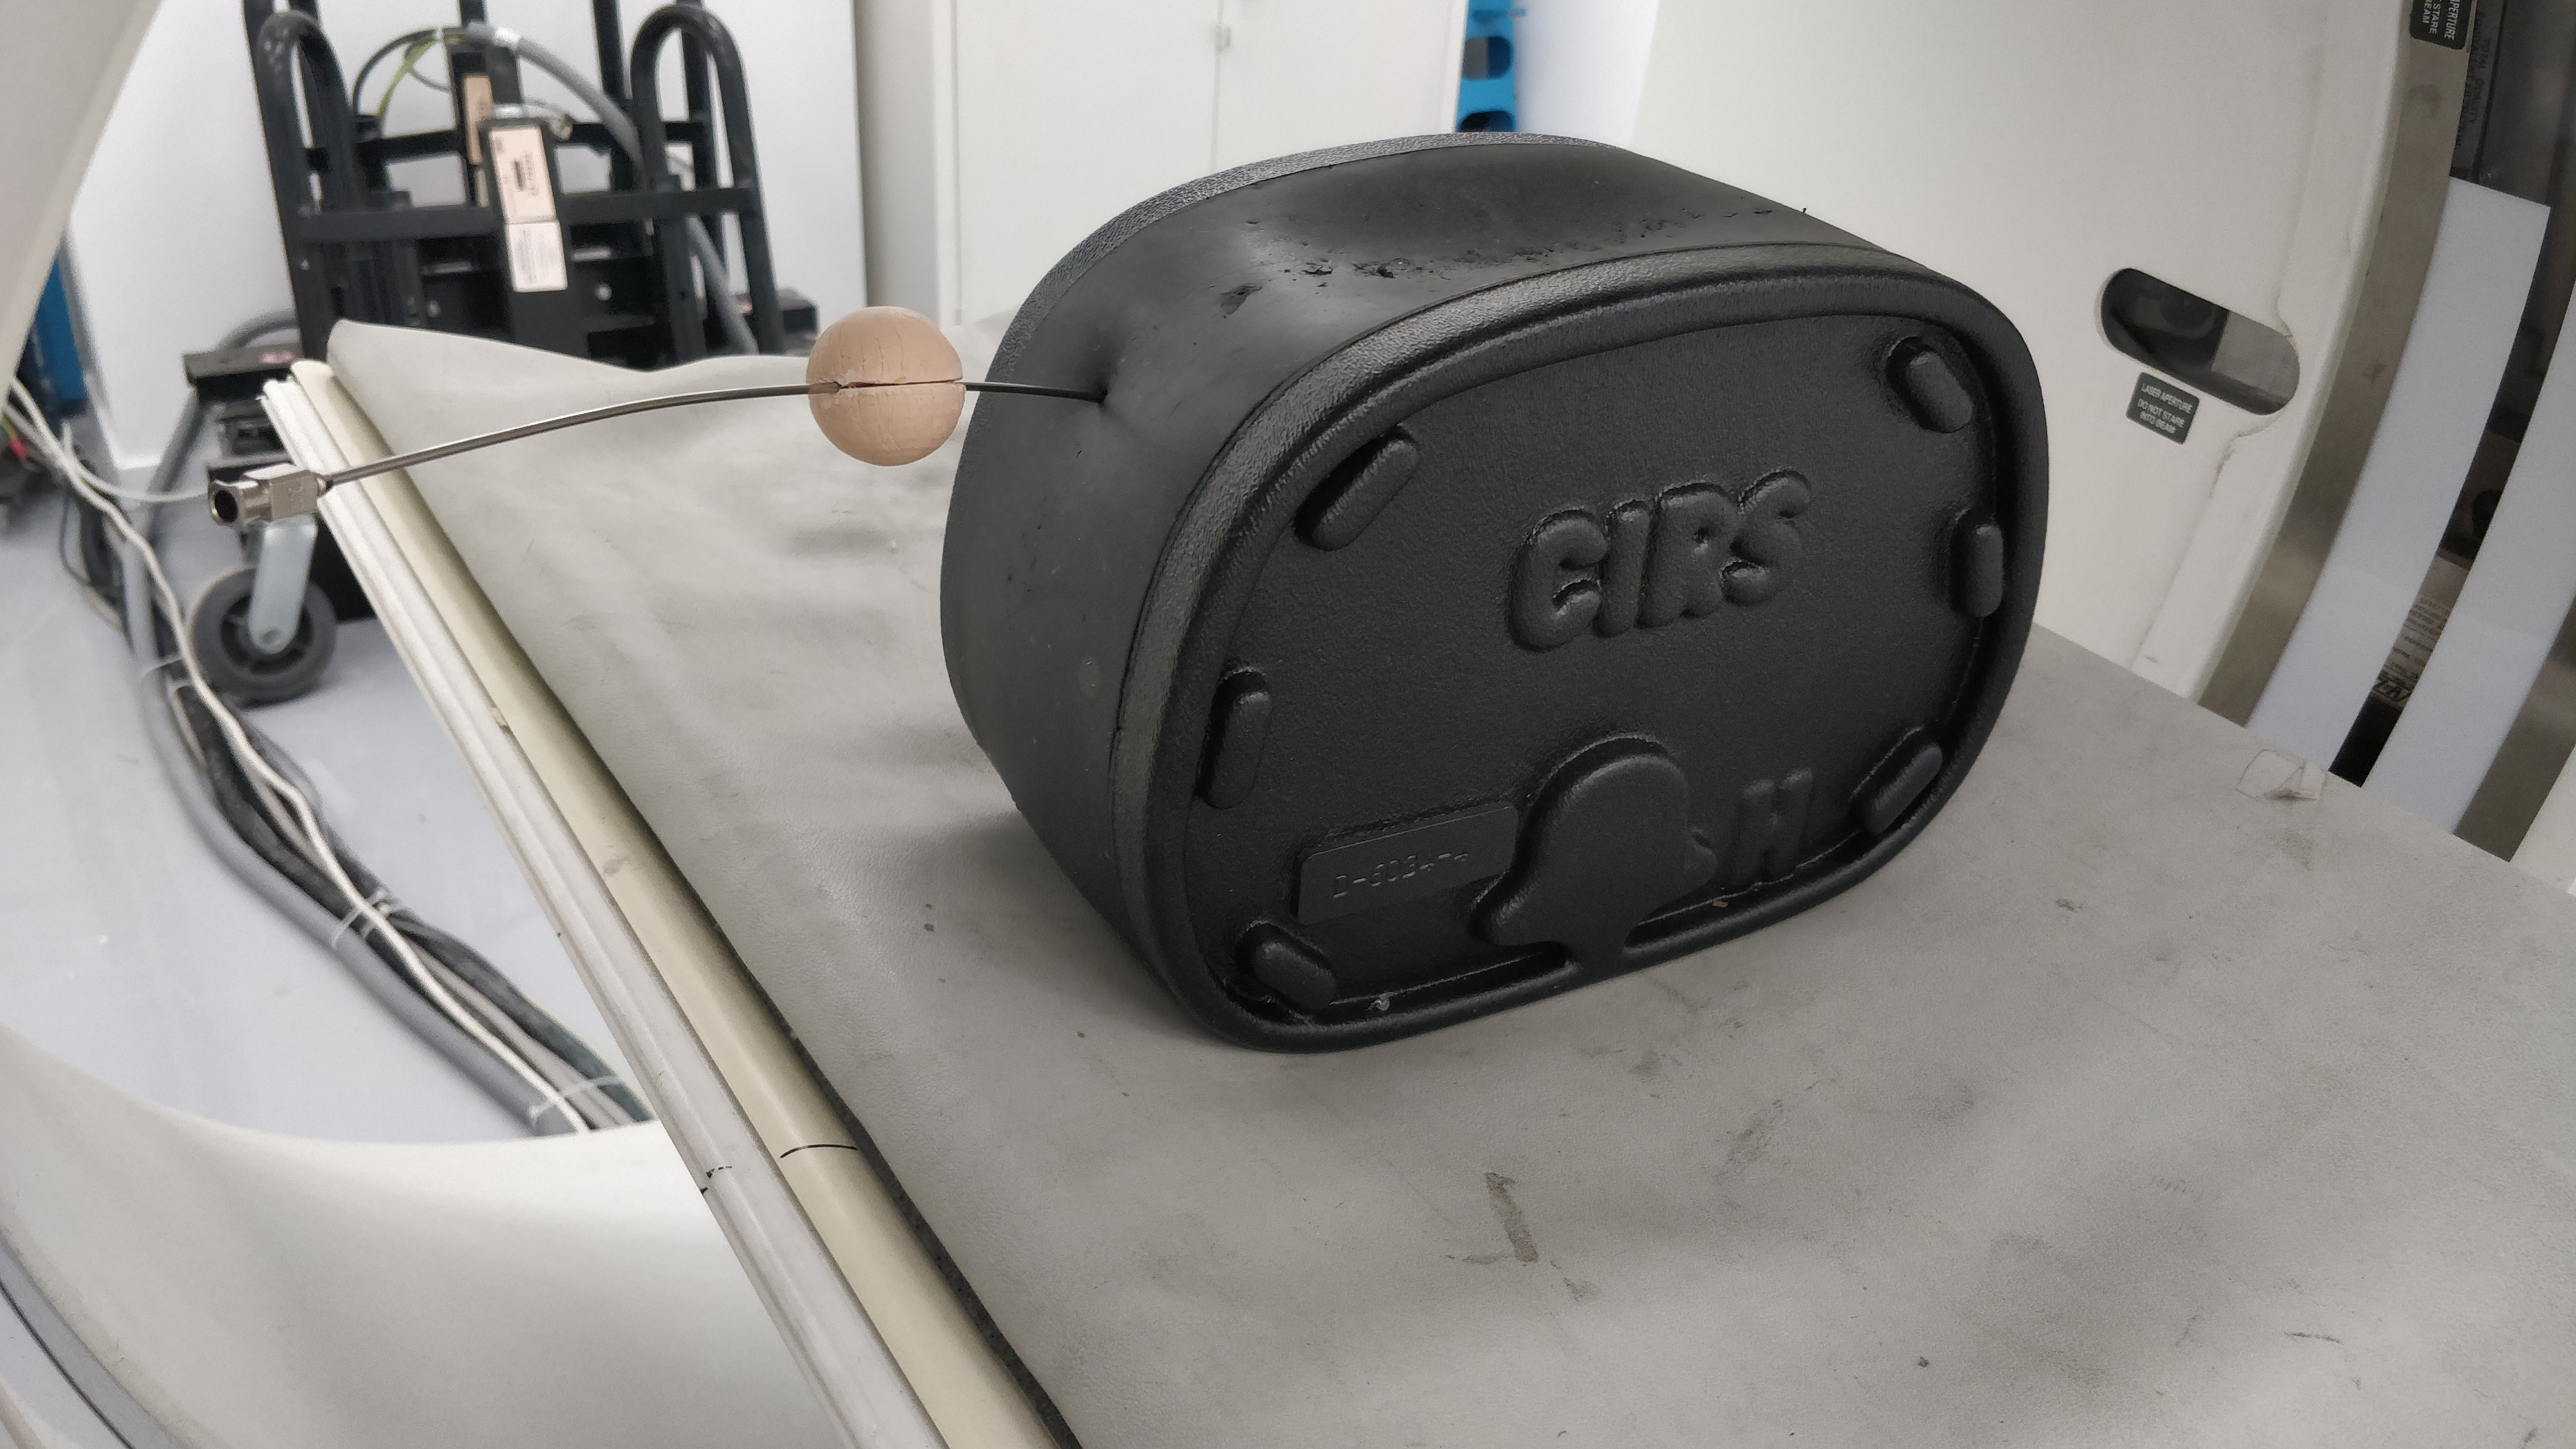
\includegraphics[width=8cm]{long_needle_phantom.jpg}
\caption{\small{Photograph of the long flexible needle with spherical marker inserted into abdomen phantom lying on the CT scanner bed.}}
\label{long_needle_fig}
\end{figure}

\begin{figure}[t]
\centering
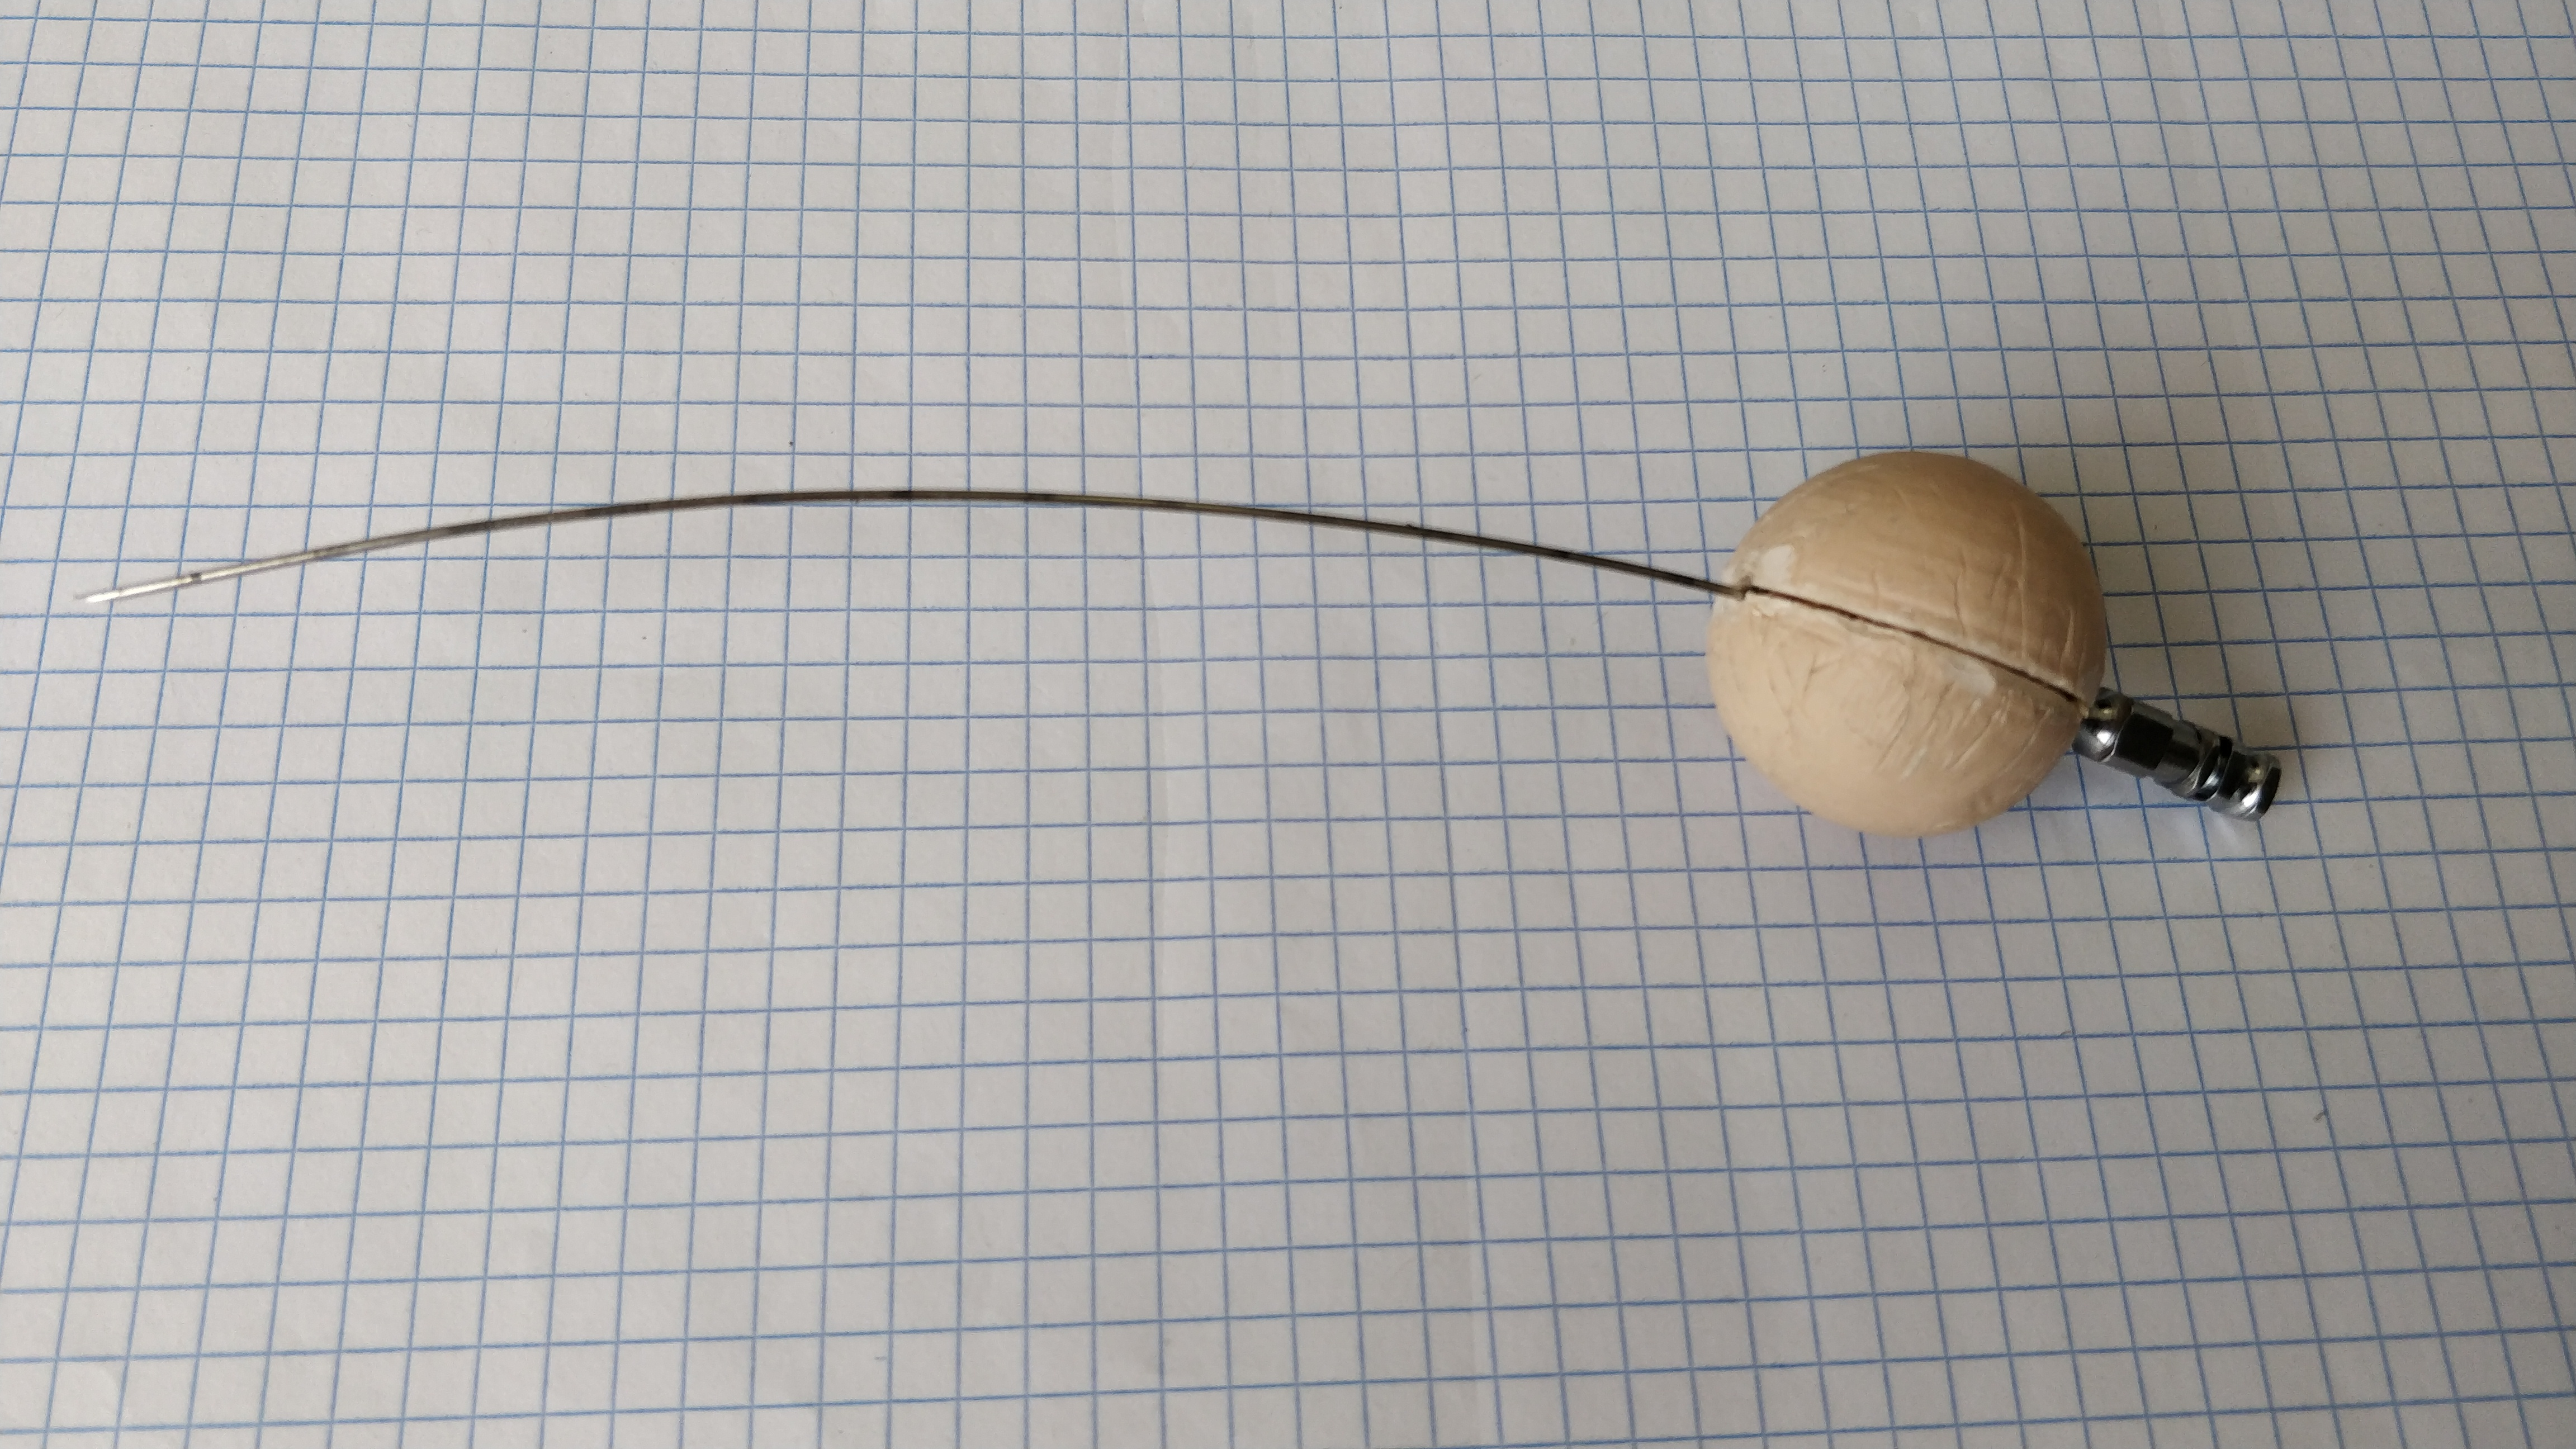
\includegraphics[width=8cm]{short_needle.jpg}
\caption{\small{Photograph of the short flexible needle with spherical marker attached at 135mm from the tip.}}
\label{short_needle_fig}
\end{figure}

\begin{figure}[b]
\centering
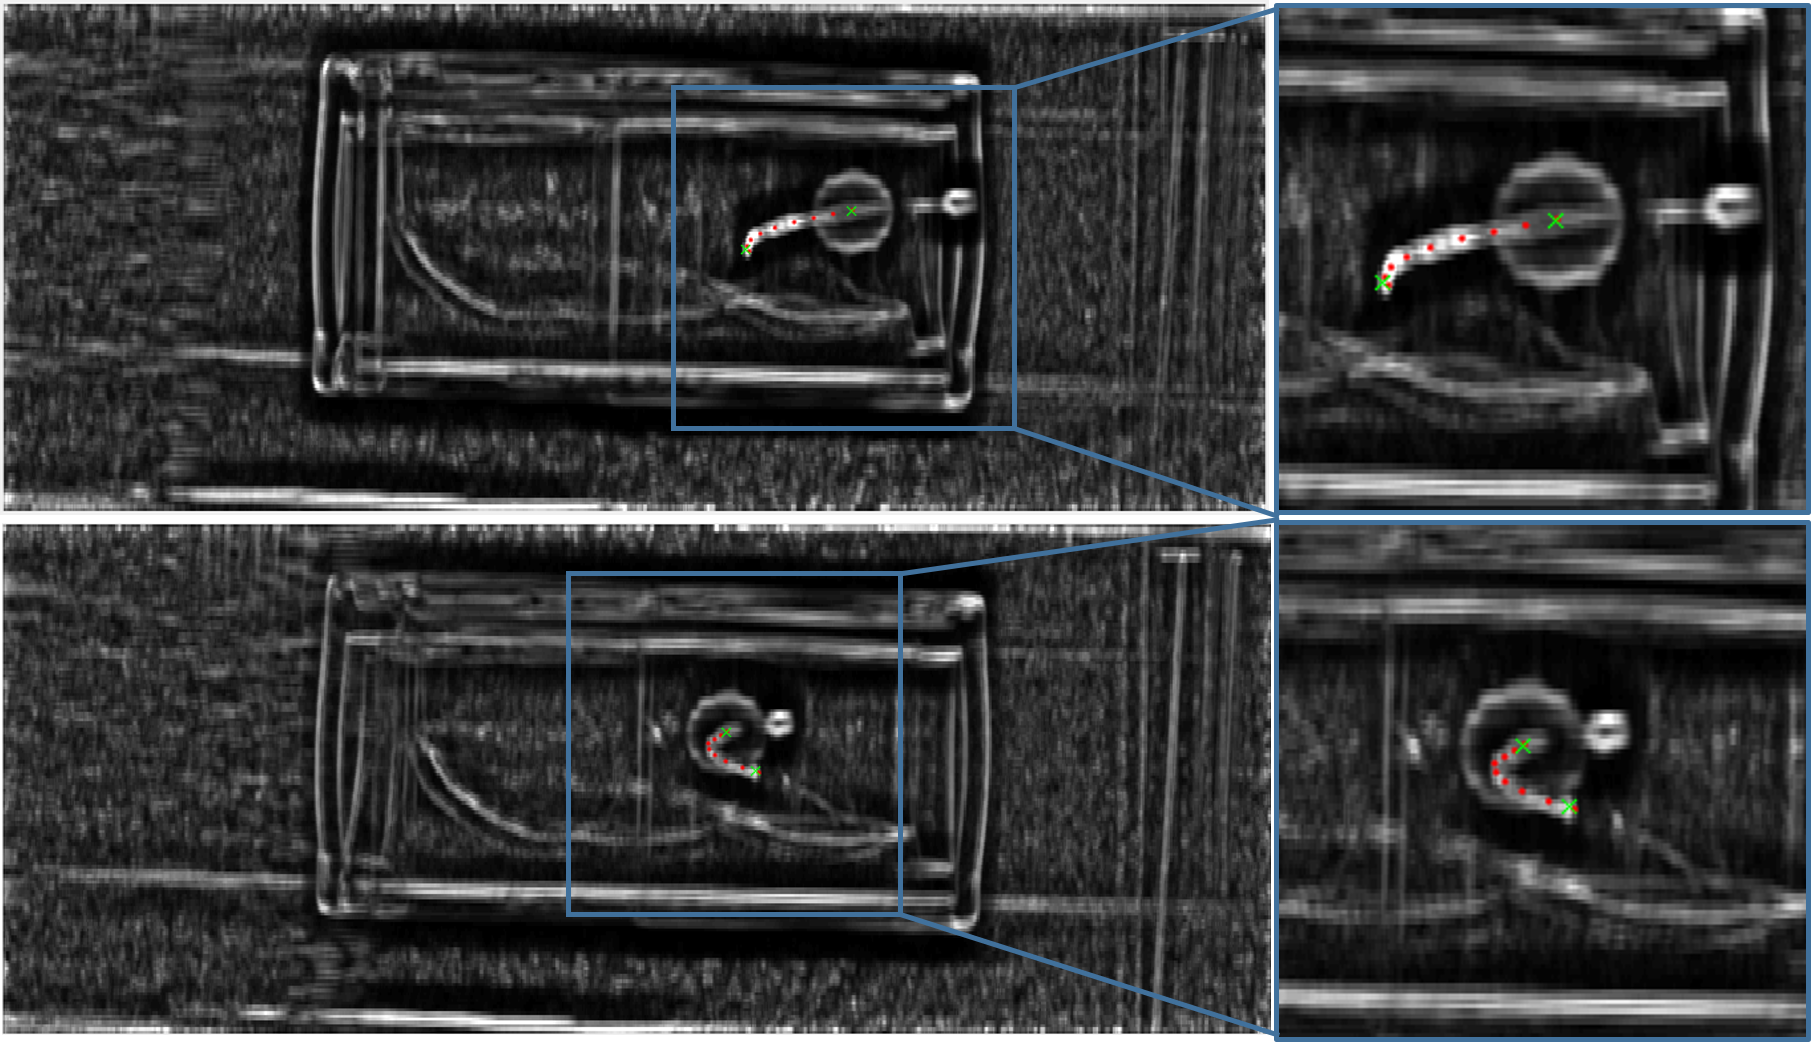
\includegraphics[width=8cm]{projection_diff_images.png}
\caption{\small{Projection difference images for two views from one scan of the short needle. the green crosses indicate ground truth center of marker and tip; red dots indicate the control points established in the incremental needle trajectory reconstruction.}}
\label{proj_diff_fig}
\end{figure}

The full baseline scan was registered to each sparse scan with needle inserted, using Radon-space rigid registration. The registration accuracy was evaluated as the root-mean-square of differences between voxel coordinates transformed by the calculated registration and by image-space registration of the reconstructed images. 
A sparse set of 24 evenly spaced view angles in the range [0$^\circ$,180$^\circ$) was used for Radon-space registration and needle path reconstruction as previous experiments \cite{medan2017reduced} with a straight needle showed this selection offered a good trade-off between robustness and potential dose reduction.
The marker center ground truth was obtained via manual localization on the reconstructed images, and the path ground truth was traced in 3D image space by a similar method to the one described above for projection space - namely, incremental tracing of short segments to establish control points based on difference image, and bezier curve reconstruction in 3D. The tip ground truth was determined as the point on the needle trace found at the known tip-marker distance. The trajectory error was evaluated as the root-mean-squared distance of points along the reconstructed curve to the nearest point on the ground-truth curve.

Table \ref{results_table} summarizes the results of needle tip localization for the 7 scans in the dataset. One of the scans (L3) shows a large tip localization error due to the needle trajectory being very close to in-plane with the axial plane (see fig. \ref{multislices_fig}). In our method, long needle segments that are in-plane lead to inaccurate estimation of the trajectory since the projections of such segments are observed as horizontal lines in the projection difference images regardless of the orientation withing the plane. This imposes a limitation encountered previously in our work on straight needles \cite{medan2017reduced}, where in-plane insertion of the needle should be avoided to enable the recovery of the needle orientation as an intersection of non-parallel planes.

Running times of 200-250 seconds were observed on Intel i7 CPU running unoptimized Matlab code. To allow our method to be used in a clinical setting, parallelization of computations on GPU will be required in order to bring the running time down to several seconds. In the projection difference calculation stage, the projection difference images can be calculated in parallel. Additionally, in each round of control point addition, the operations on each projection difference image can be parallelized to further reduce the running time.

\section{Discussion}
Our method extends the novelty of imageless projection-space localization from rigid to flexible needles, allowing the potential of dose reduction in a larger range of interventional CT procedures. The localization can be displayed as visual feedback to the radiologist on the baseline scan, which is free from artifacts due to the needle, allowing an unobstructed view of the target tissue.

\begin{figure*}
\centering
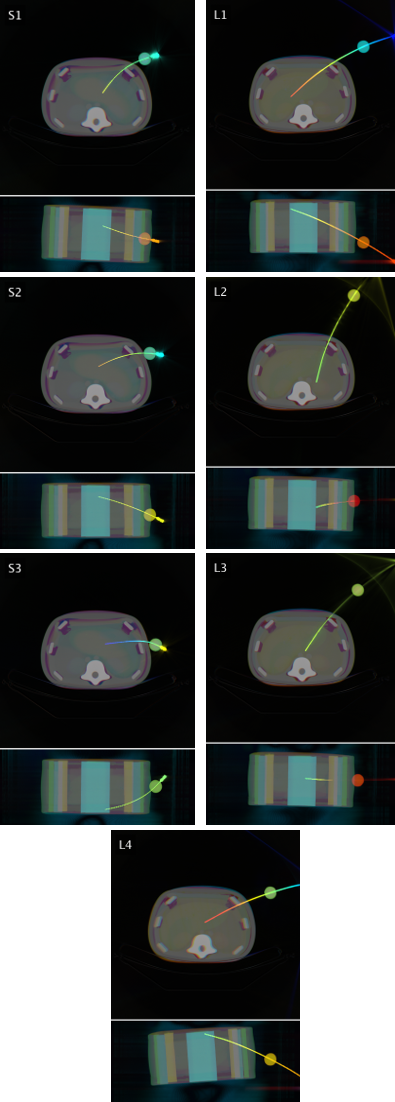
\includegraphics[width=\textwidth]{multislices.png}
\caption{\small{Axial and coronal multi-slice views (top and bottom of each sub-image, respectively) of the abdomen phantom with flexible needle (L-long, S-short) inserted in different positions. The multi-slice views are generated by assigning a color map to encode the depth of each slice in the direction perpendicular to the image plane.}}
\label{multislices_fig}
\end{figure*}

Visual feedback is particularly important for robotically driven needles, where the interaction of the needle and tissue is modeled in order to construct a control sequence realizing a planned insertion path. Such systems would benefit from mid-insertion feedback that would allow adjustments to the control sequence based on the achieved state of the needle insertion, and a reduction in x-ray dose will benefit the patient who will be subjected to a smaller radiation-related risk.


Our method is suitable when the baseline and repeat scans have minimal deformations and rigid registration can be used to align them. The scan field of view needs to includes the flexible needle and the spherical marker, while keeping the insertion out-of-plane.

The study itself is limited to several scans of an abdomen phantom, with the fractional scanning simulated from full scans by omitting most of the repeat scan data used as input for the algorithm. To implement our method on a commercial CT scanner, fractional scanning would have to be achieved by one of two possible approaches: fast modulation of the x-ray tube current and/or voltage, or fast mechanical collimation during acquisition. Such methods would require hardware integration beyond the scope of this work, but since the fraction of views required in the repeat scan is below 5\%, there is potential for substantial dose reduction.


\section{Conclusions}
We have described a flexible needle extension of our method for needle and patient tracking in interventional CT procedures, based on fractional CT scanning without image reconstruction.
Our method accurately traces a flexible needle's 3D trajectory by following its path in projection space for a sparse set of views. Starting from a spherical marker attached to it at a known distance from the tip, it traces the path to the tip without reconstructing the CT image.

The main advantages of our method are:
1) accurate flexible needle trajectory and needle tip localization without image reconstruction;
2) significant potential dose reduction for each individual repeat scan localization;
3) simultaneous patient registration and needle localization for every snapshot; 
4) fully automatic, no calibration and/or manual setup;
5) only a simple marker attached to the needle is required; 
6) artifact-free monitoring of a flexible needle's trajectory on top of a baseline scan.

An accuracy level comparable to 3D image space methods is shown in our experimental results.
The dose reduction enabled by our method allows either more frequent tip localizations during needle insertion for a similar total dose, or a reduced total dose for the same frequency of tip localization.

%%%%%%%%%%%%%%%%%%%%%%%%%%%%%%%%%%%%%%%%%%%%%%%%%%%%%%%%%%%%%%%%%%%%%%%%%%%%%%%%

%\addtolength{\textheight}{-15cm} % This command serves to balance the column lengths
      % on the last page of the document manually. It shortens
      % the textheight of the last page by a suitable amount.
      % This command does not take effect until the next page
      % so it should come on the page before the last. Make
      % sure that you do not shorten the textheight too much.

\bibliographystyle{ieeetr}
\bibliography{flexible_needle}

\end{document}
